\section{Machine Learning based Method}

For the machine learning method, WEKA, developed at the University of Waikato in New Zealand, was chosen as the library. As described by Witten et al., "[t]he WEKA workbench is a collection of machine learning algorithms and data preprocessing tools [...]" \cite[p.~7]{weka}. It also includes tools for the entire process of data mining, such as preparation of data and evaluation. WEKA is implemented in Java, the version of the library used in this thesis was 3.9.6. It also offers a graphical interface, which was not used in this thesis, only the library was used \cite{weka}. Weka was chosen because of its large collection of both algorithms and tools for data mining, as well as ease of use through an extensive documentation.

Weka uses the Attribute-Relation File Format for its data, which contains a header describing the attributes, as well as the data itself, with one row containing one instance \cite{weka}. For this thesis, the class attribute was chosen to be nominal, either negative (-1.0) or positive (1.0), so we have a binary classification problem. Furthermore, the tweet text is added as a string attribute.

\TODO{Twitter API for test data?}
\subsection{Training data}
The training data for machine learning classifiers was created by Go et al. and consists of 1.6 million tweets \cite{GoBHaHua2009}. The tweets were parsed using the Twitter API by querying for positive or negative emoticons, such as ":)" and labeled as positive or negative depending on the emoticon. Furthermore, tweets containing both a negative and positive emoticon, as well as retweets were removed \cite{GoBHaHua2009}.

This resulted in 800,000 positive and 800,000 negative tweets that were periodically requested on no specific topic, thus covering a large number of topics \cite{GoBHaHua2009}.

\TODO{delete parts that are methodology, only specifics/implementation details.}

\subsection{Tokenization}
For Tokenization, weka's WordTokenizer was used, with the default delimiters, such as whitespace and "\textbackslash n".
\subsection{Stop Word Filtering}
For Stop Word Filtering, both a list and a dynamic approach were used. A short list of common words such as "the" was manually collected and evaluated. To further reduce the word size, a limit was set for how often a word has to appear to be used as well as a (soft) limit of total words. In the testing, a limit of 15,000 words was found to be optimal, with words appearing at least 20 times in the training data. This allowed for the greatest balance of performance and accuracy. This limit was set in weka's StringToWordVector, which is explained in more detail later.
\subsection{URL/Hashtag Removal}
??

\subsection{Stemming}
For stemming, weka's LovinsStemmer was used, which is based on the Lovins Stemmer \cite{weka}. This stemmer uses a two-step method, which first removes the ending, thus obtaining the stem. After this, similar stems are combined to account for different spellings. An example for this is "absorption", whose stem is "absorpt", while "absorbing" will result in "absorb"\cite{Lovins1968DevelopmentOA}.

\subsection{Feature Selection}
In order to transform the text of a tweet into a suitable format for classifiers, weka's StringToWordVector filter is used \cite{weka}. This filter transforms the string feature, the tweet's text, by parsing each word out of it using the previously defined WordTokenizer. The words are then added to a dictionary, which stores all recognized words. In the data, the words are implemented as numeric attributes, with the value denoting the number of occurrences or its presence.

For example, the tweet "i love it" would result in three attributes, the attribute "i", the attribute "love", and the attribute "it", as can be seen in Figure \ref{fig:arff_train}. The dictionary, and with it the attributes, are all determined by the training data. The test data is also filtered, but only using the known words from the training data, no new words are added. 




\begin{figure}
    \centering
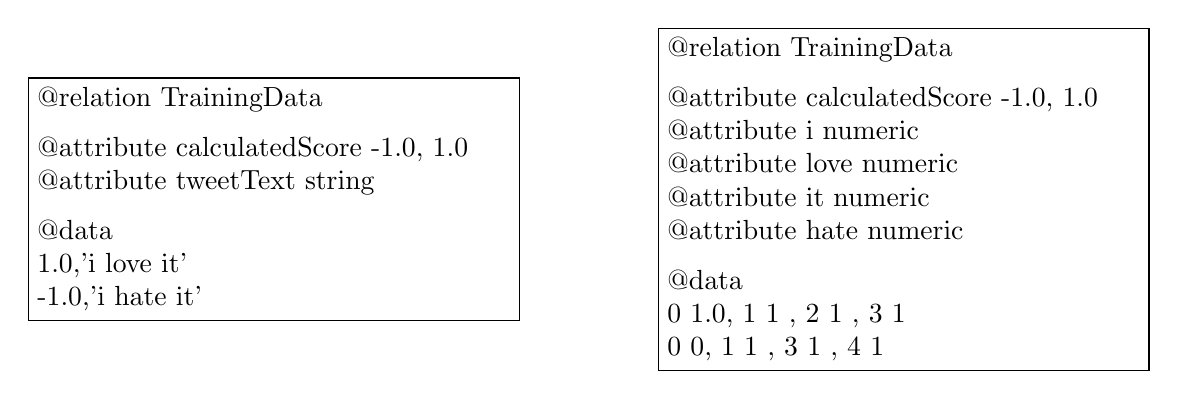
\begin{tikzpicture}
\vspace{5mm}
\node[draw, text width=6cm] at (0,0) { @relation TrainingData \\
                                        \medskip
                                        @attribute calculatedScore {-1.0, 1.0} \\
                                        @attribute tweetText string \\
                                        \medskip
                                        @data \\
                                        1.0,'i love it' \\
                                        -1.0,'i hate it' \\
                                        
                                        };
\node[draw, text width=6cm] at (8,0) { @relation TrainingData \\
                                        \medskip
                                        @attribute calculatedScore {-1.0, 1.0} \\
                                        @attribute i numeric \\
                                        @attribute love numeric \\
                                        @attribute it numeric \\
                                        @attribute hate numeric \\
                                        \medskip
                                        @data \\
                                        {0 1.0, 1 1 , 2 1 , 3 1} \\
                                        {0 0,   1 1 , 3 1 , 4 1}
                                        };
\end{tikzpicture}
\vspace{5mm}
    \caption{Example of training data in the ARFF format utilized by Weka before and after feature selection \cite{weka}.}
    \label{fig:arff_train}
\end{figure}


\subsection{Training}
\TODO{actual implementation stuff}
